% Experiment 3: two square MCMC convergence graphs, package multivariate style.
% Solid black: agree on every monitored parameter.
% Dashed: agree on some parameters only.
\begin{figure}[H]
\centering
\rule{\textwidth}{0.4pt}\\[3pt]
\setlength{\tabcolsep}{0pt}
\begin{tabular}{@{}cc@{}}
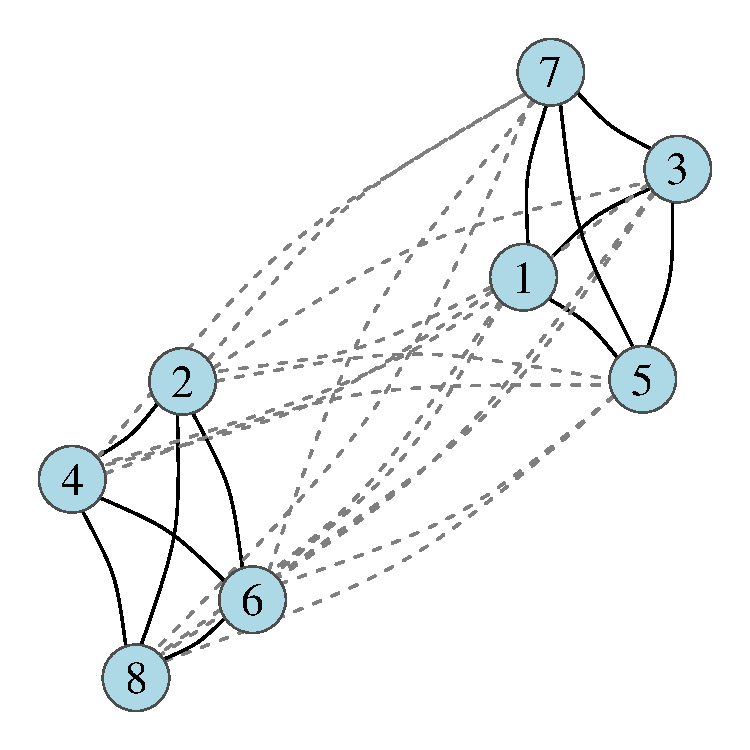
\includegraphics[width=4cm,height=4cm]{fig_experiment3_a_all_parameters.pdf} &
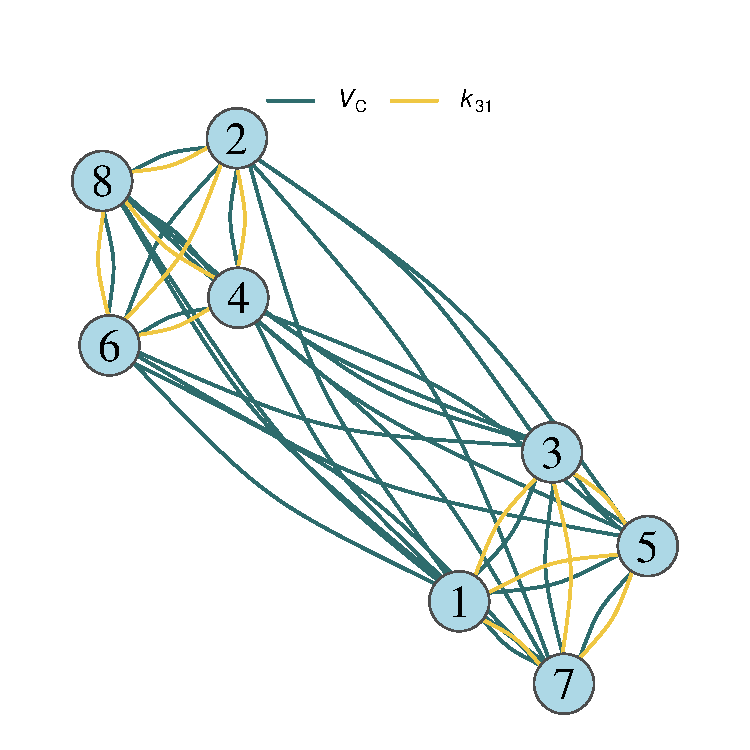
\includegraphics[width=4cm,height=4cm]{fig_experiment3_b_k31_VC.pdf}
\end{tabular}\\[3pt]
\rule{\textwidth}{0.4pt}
\caption{%
\textbf{MCMC convergence graphs for the three-compartment
pharmacokinetic model.}
Solid black edges belong to $G_\cap$ (agree on every monitored parameter).
Dashed edges belong to $G_\cup\setminus G_\cap$ (agree on some parameters only).
The left panel monitors $k_{10}$, $k_{12}$, $k_{21}$, $k_{13}$, $k_{31}$ and $V_C$.
The right panel monitors $k_{31}$ and $V_C$:
solid edges agree on both parameters;
dashed edges agree on one parameter only.
Teal is $V_C$ and yellow is $k_{31}$.
}
\label{fig:experiment3-graphs}
\end{figure}
